%----------------------------------------------------------------------------------------
%   PHẦN 1: GIỚI THIỆU ĐỀ TÀI
%----------------------------------------------------------------------------------------
\section{Giới thiệu đề tài}

\begin{frame}{Bối cảnh giao thông Việt Nam 2025}
    \begin{itemize}
        \item Đô thị hóa và chuyển đổi số mạnh tại Hà Nội, TP. Hồ Chí Minh.
        \item ITS và camera phạt nguội bắt đầu triển khai nhưng còn phân tán.
        \item Giao thông hỗn hợp, mật độ xe máy cao, vi phạm phổ biến.
    \end{itemize}
    \begin{alertblock}{Thách thức chính}
        \begin{itemize}
            \item Chi phí hệ thống AI nhập ngoại cao, khó mở rộng đại trà.
            \item Điều kiện ánh sáng thay đổi, che khuất, góc quay nghiêng.
            \item Nhu cầu làm chủ công nghệ phù hợp đặc thù Việt Nam.
        \end{itemize}
    \end{alertblock}
\end{frame}

\begin{frame}{Bài toán nhận diện biển số xe}
    \begin{itemize}
        \item ALPR là thành phần quan trọng trong ETC, bãi đỗ, an ninh và giám sát vi phạm.
        \item Biển số Việt Nam có định dạng đặc thù, chất lượng ảnh không đồng đều.
        \item Yêu cầu: chính xác, thời gian thực, chi phí triển khai thấp.
    \end{itemize}
\end{frame}

\begin{frame}{Mục tiêu đề tài}
    \begin{block}{Mục tiêu chính}
    Xây dựng hệ thống giám sát giao thông thông minh với các chức năng:
    \begin{itemize}
        \item \textbf{Phát hiện} đa loại phương tiện (5 lớp).
        \item \textbf{Theo dõi} quỹ đạo liên tục và đếm lưu lượng.
        \item \textbf{Nhận diện biển số} xe Việt Nam (ALPR).
        \item \textbf{Phát hiện vi phạm} (vượt đèn đỏ, đi sai làn).
    \end{itemize}
    \end{block}

    \begin{block}{Yêu cầu kỹ thuật}
    \begin{itemize}
        \item Xử lý thời gian thực trên phần cứng phổ thông.
        \item Độ chính xác cao, vận hành ổn định.
        \item Giao diện trực quan, dễ cấu hình ROI/làn đường.
    \end{itemize}
    \end{block}
\end{frame}

\begin{frame}{Kiến trúc tổng quát hệ thống}
    \begin{block}{Luồng xử lý (Data Pipeline)}
    \centering
    \textbf{Video Input} $\rightarrow$ \textbf{Detection} $\rightarrow$ \textbf{Tracking} $\rightarrow$ \textbf{ALPR} $\rightarrow$ \textbf{Violation Check}
    \end{block}

    \vspace{0.4em}
    \textbf{4 module chính:}
    \begin{enumerate}
        \item \textbf{Vehicle Detection:} YOLOv8n (5 lớp phương tiện)
        \item \textbf{Multi-Object Tracking:} ByteTrack
        \item \textbf{License Plate Recognition:} YOLO + PaddleOCR
        \item \textbf{Violation Detection:} Logic Engine (vượt đèn đỏ, sai làn)
    \end{enumerate}
\end{frame}

\section{Cơ sở lý thuyết: Phát hiện \& Theo dõi}

\begin{frame}{Tổng quan về Phát hiện đối tượng}
    \begin{itemize}
        \item \textbf{Định nghĩa:} Xác định vị trí và phân loại các thực thể quan tâm trong ảnh/video.
        \item \textbf{Đầu ra:} Tập bounding box $B = \{b_1, b_2, \dots, b_N\}$:
        $$ b_i = (x_i, y_i, w_i, h_i, c_i, p_i) $$
        \item $(x_i, y_i)$: tọa độ tâm; $(w_i, h_i)$: kích thước; $c_i$: lớp; $p_i$: độ tin cậy.
        \item \textbf{Thách thức:} biến thiên tỉ lệ, che khuất, ánh sáng thay đổi.
    \end{itemize}
\end{frame}

\begin{frame}{Cơ chế chia lưới \& biểu diễn đầu ra (YOLO)}
    \begin{figure}
        \centering
        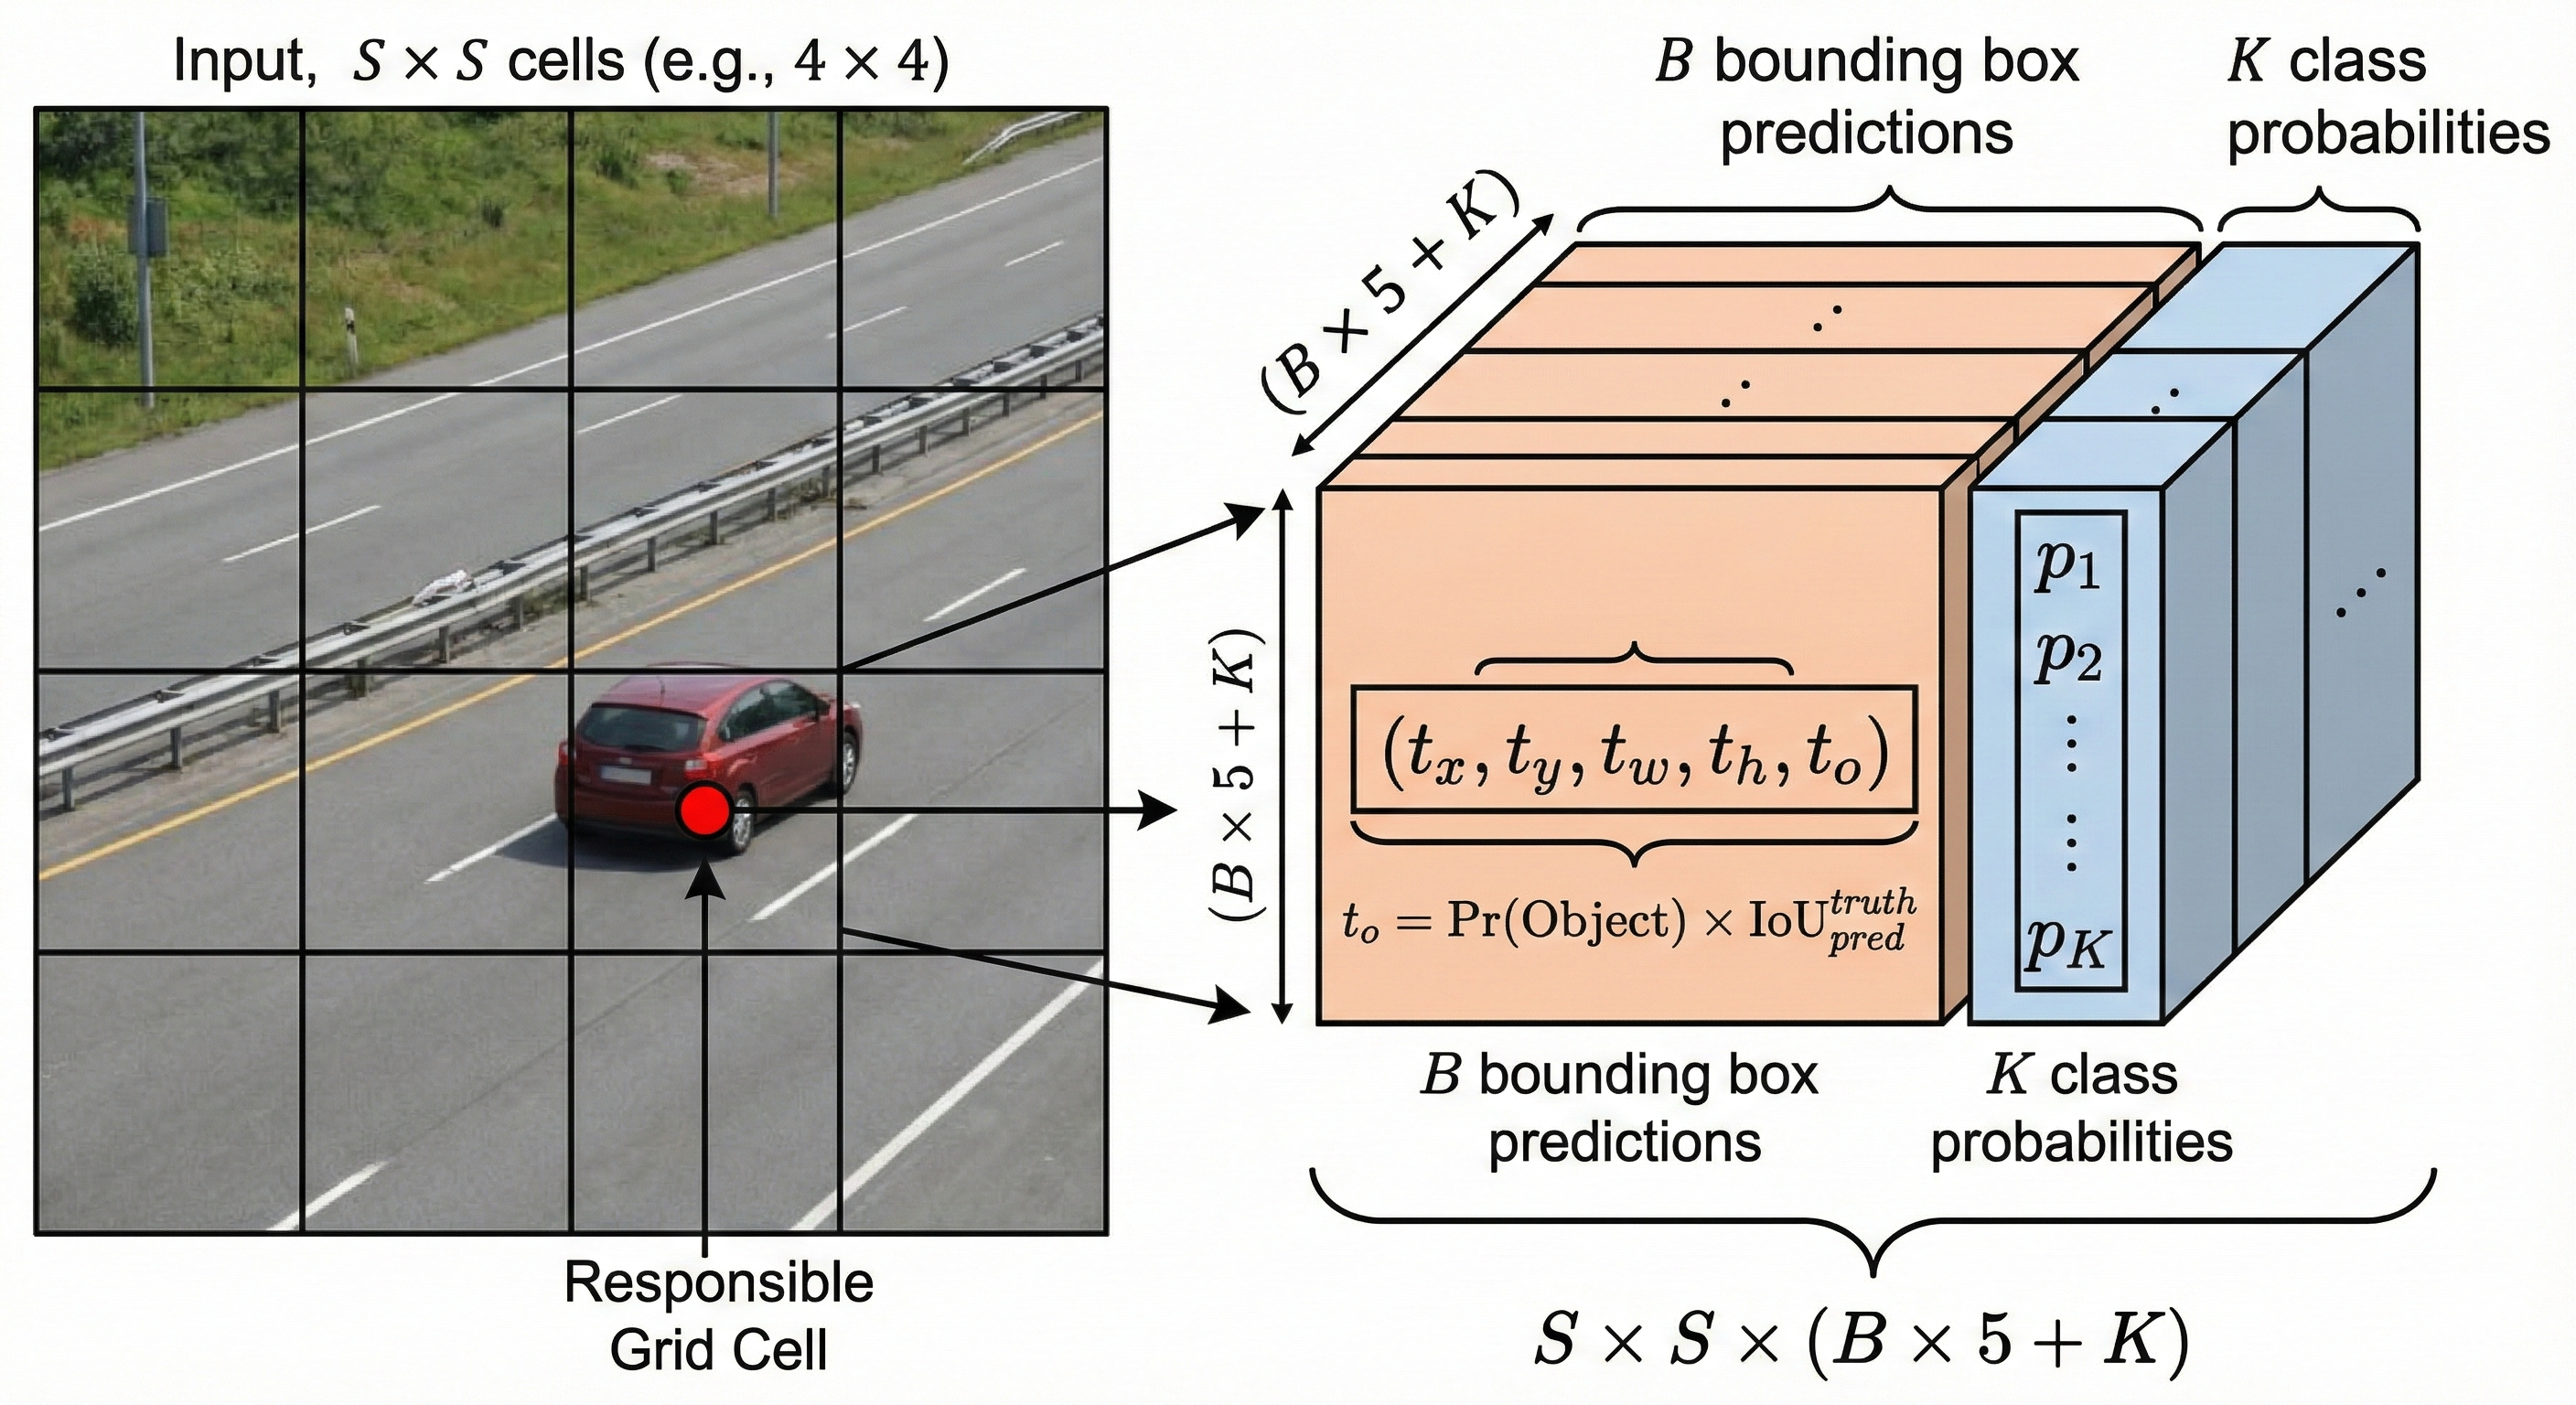
\includegraphics[width=0.75\linewidth]{Figures/chia_luoi.png}
        \caption{Cơ chế chia lưới và biểu diễn đầu ra của YOLO}
    \end{figure}
\end{frame}

\begin{frame}{Lựa chọn mô hình: YOLOv8}
    \textbf{Lý do lựa chọn YOLOv8 cho bài toán giao thông:}
    \begin{itemize}
        \item \textbf{Anchor-free:} Linh hoạt với đối tượng có tỉ lệ biến thiên lớn.
        \item \textbf{Module C2f:} Trích xuất đặc trưng giàu thông tin, nhẹ.
        \item \textbf{Task Aligned Assigner:} Cân bằng giữa phân loại và định vị.
        \item \textbf{Hiệu năng:} Tốc độ cao, phù hợp real-time.
    \end{itemize}
\end{frame}

\begin{frame}[allowframebreaks]{Kiến trúc mạng YOLOv8}
    Hệ thống gồm 3 thành phần chính:
    \begin{enumerate}
        \item \textbf{Backbone (CSPDarknet cải tiến):} Trích xuất đặc trưng với C2f, SPPF.
        \item \textbf{Neck (PANet):} Kết hợp đặc trưng đa tỉ lệ.
        \item \textbf{Head (Decoupled):} Tách nhánh phân loại và hồi quy hộp.
    \end{enumerate}
    \framebreak
    \begin{figure}
        \centering
        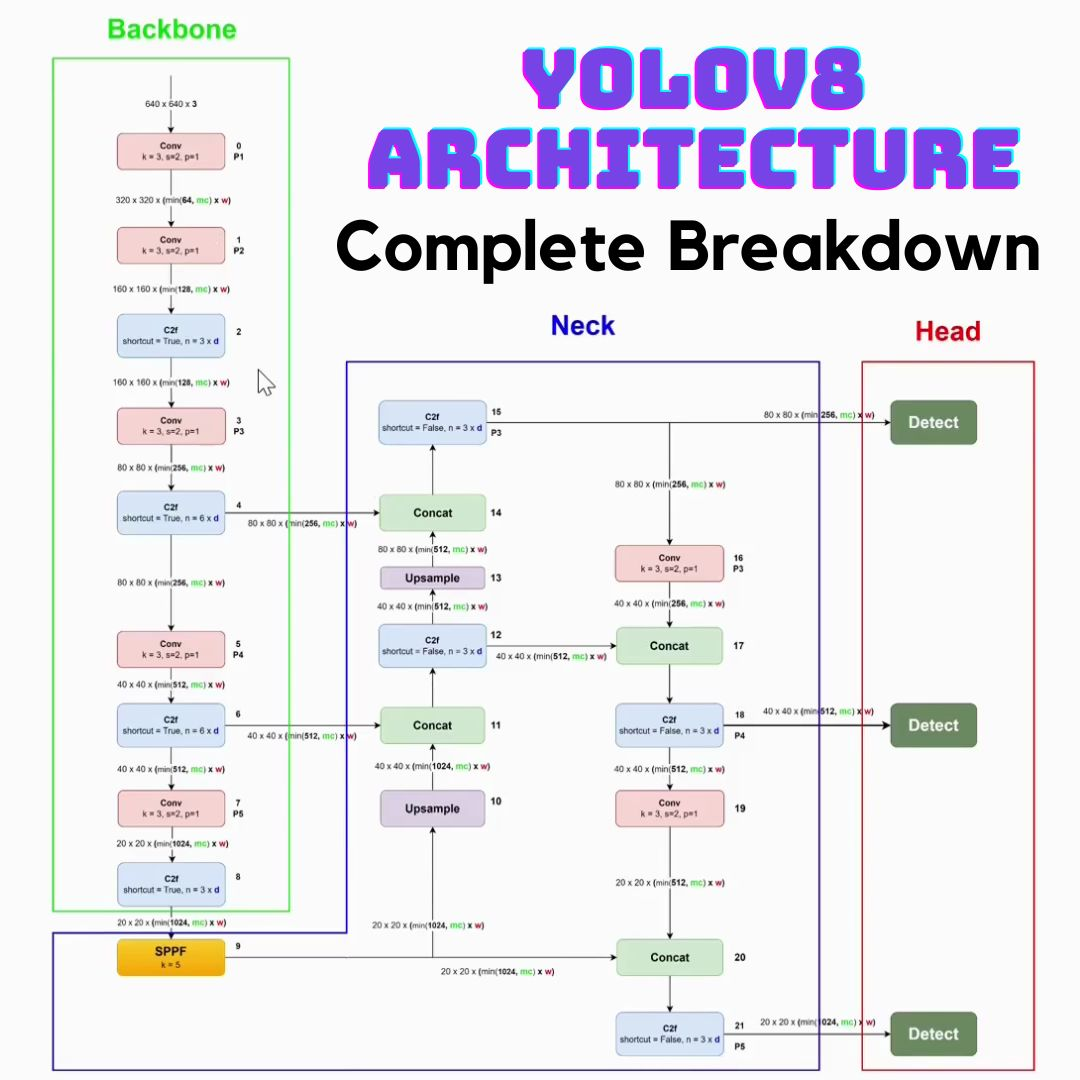
\includegraphics[width=0.65\linewidth]{Figures/1698478493766.jpg}
    \end{figure}
\end{frame}

\begin{frame}{Hàm mất mát trong YOLOv8}
    Tối ưu hóa hàm mất mát tổng hợp:
    $$ L_{total} = \lambda_{box} L_{box} + \lambda_{cls} L_{cls} + \lambda_{dfl} L_{dfl} $$
    \begin{block}{Thành phần chính}
    \begin{itemize}
        \item \textbf{CIoU Loss} cho định vị khung.
        \item \textbf{DFL} cho chất lượng biên khung.
        \item \textbf{VFL/BCE} cho phân loại.
    \end{itemize}
    \end{block}
\end{frame}

\begin{frame}{Theo dõi đa đối tượng (MOT)}
    \textbf{Mục tiêu:} Gán ID duy nhất cho mỗi đối tượng qua các khung hình.
    \begin{itemize}
        \item \textbf{Kalman Filter:} Dự đoán vị trí/động học.
        \item \textbf{Hungarian Algorithm:} Ghép cặp detection và track tối ưu.
        \item \textbf{Tracking-by-Detection:} Dựa trên kết quả YOLOv8.
    \end{itemize}
\end{frame}

\begin{frame}[allowframebreaks]{Thuật toán ByteTrack}
    \textbf{Ý tưởng:} Tận dụng mọi detection, kể cả điểm tin cậy thấp.
    \begin{enumerate}
        \item \textbf{Giai đoạn 1 (High Score Matching):}
        Ghép detection chất lượng cao với track hiện có (IoU + Kalman).
        \item \textbf{Giai đoạn 2 (Low Score Matching):}
        Ghép các track chưa khớp với detection điểm thấp để “cứu” ID.
    \end{enumerate}
    \textit{Ưu điểm:} Tốc độ cao, ổn định khi che khuất.
    \framebreak
    \begin{figure}
        \centering
        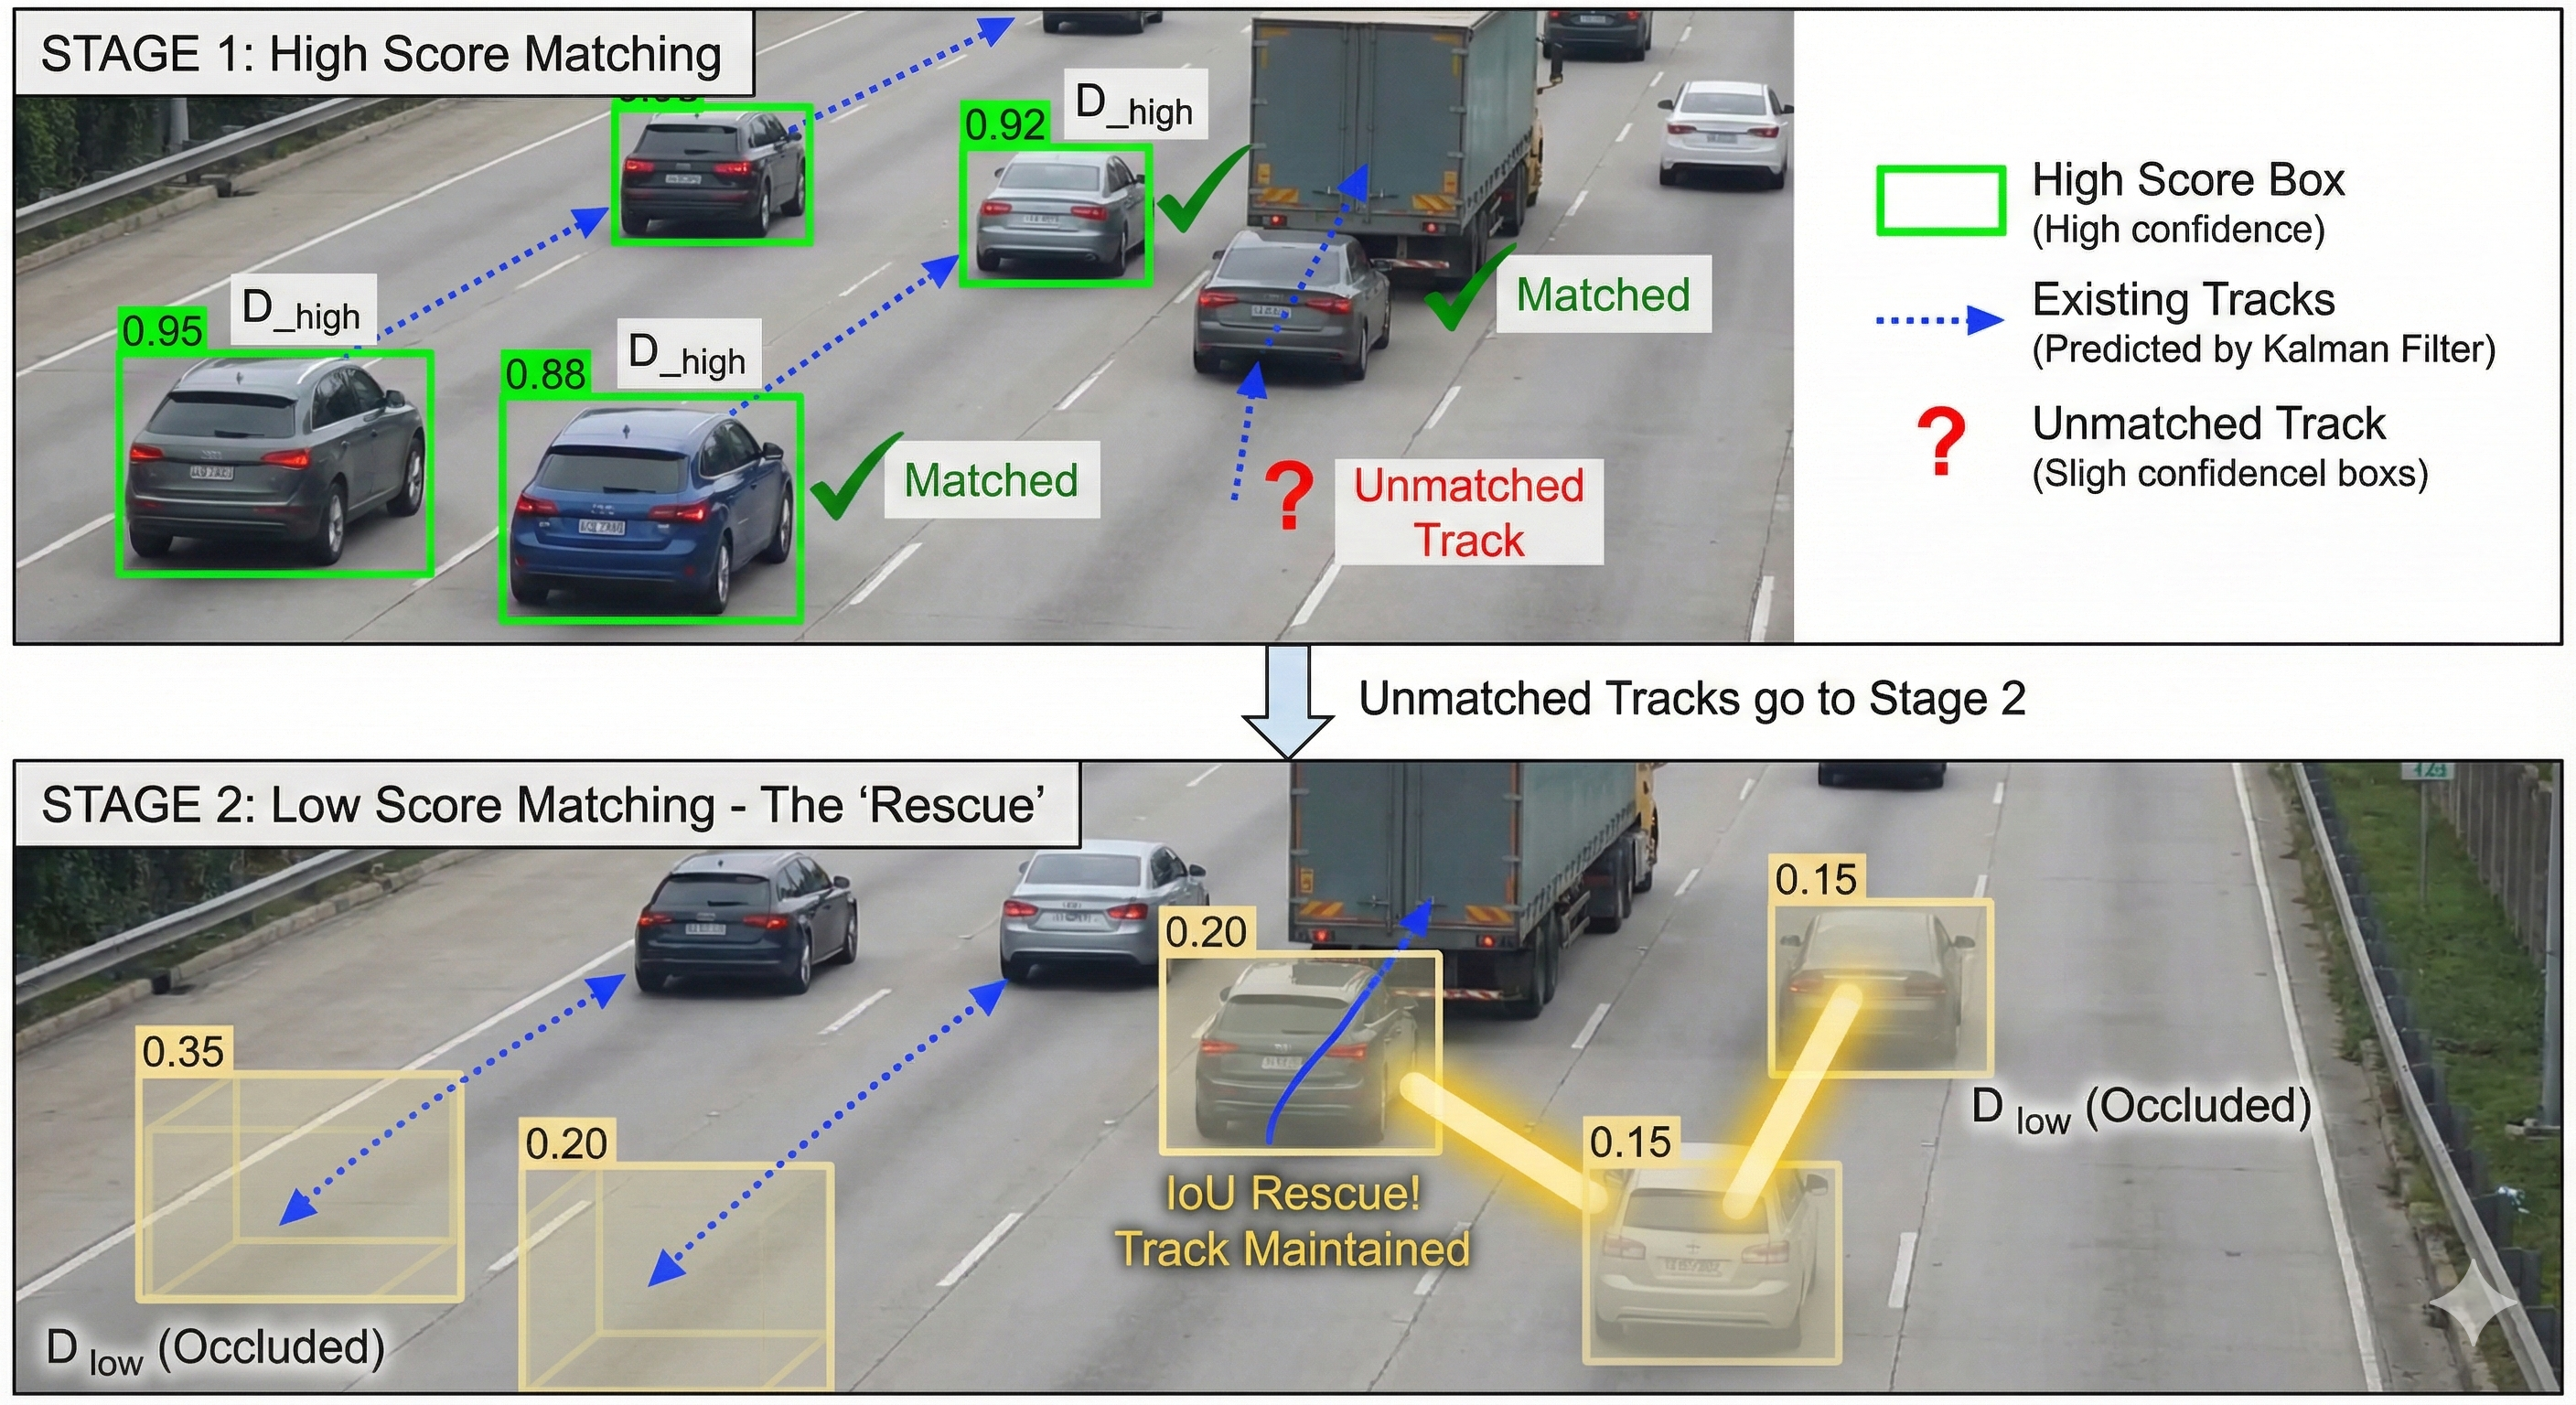
\includegraphics[width=0.75\linewidth]{Figures/bytetrack.png}
        \caption{Minh họa cơ chế liên kết hai giai đoạn của ByteTrack}
    \end{figure}
\end{frame}

\begin{frame}[allowframebreaks]{Xử lý ảnh \& Hình học tính toán}
    \begin{block}{Nhận diện đèn (HSV)}
        Chuyển RGB $\to$ HSV để tách màu và độ sáng.
        \begin{itemize}
            \item \textbf{Đỏ:} $H \in [0,10] \cup [160,180]$
            \item \textbf{Vàng:} $H \in [20,35]$
            \item \textbf{Xanh:} $H \in [40,85]$
            \item Voting theo tỉ lệ pixel để quyết định trạng thái đèn.
        \end{itemize}
    \end{block}
    \framebreak
    \begin{block}{Hình học tính toán}
        \begin{itemize}
            \item \textbf{Point-in-Polygon:} Xác định xe thuộc làn/ROI.
            \item \textbf{Stopline:} Tính khoảng cách tới vạch dừng để phát hiện cắt qua.
            \item \textbf{Hướng di chuyển:} So sánh vector chuyển động với vector tham chiếu để phân loại đi thẳng/rẽ.
        \end{itemize}
    \end{block}
\end{frame}
